\unfinished{Write background}

\subsection{Generalized Deduplication}
Deduplication is a technique to perform compression in storage systems. The technique works by utilizing the simarlity of file chunks. Each unique file chunk is stored once. Subsequent copies of the chunks are then replaced with a reference to the stored chunk. The method is established and shown to have good compression gain on various practical scenarios \cite{deduplication}. However, if there are minor discrepancies in the file chunks, the technique will not leverage any of the similarities. Resulting in the near-identical chunks being stored in full. Sensor data from IoT devices is one example of the data potentially being near-identical. 

To utilize the similarities in the almost identical data, a generalization of deduplication has been studied.     
This method consider the chunks at the bit level and splits them into two parts, the \textit{base} and \textit{deviation}. The \textit{base} is the identical part that is to be stored once and herafter referenced with pointers. The \textit{deviation} is the disparity between the chunks. Looking at a simple example with four 6-bit numbers, $100000$, $100001$, $100010$ and $100011$. It can be identified that the four most significant bits of the numbers are identical. Hence, leading to all having a shared \textit{base} of $1000$. The two least significant bits are then the \textit{deviation}\cite{gen-deduplication}.   

\subsection{Isolation Forest}
Anomaly detection is a combination of outlier- and novelty detection. Including both identifying outliers in the training data and determining if unseen observations are outliers. Isolation Forest (iForest) is an anomaly detection method. It differs from other popular techniques in the way that it identifies anomalies explicitly instead of profiling ordinary data points\cite{iforest}. IForest utilizes decision trees similar to other tree ensemble methods.
The main principle is to recursively split each data point, and then evaluate the amount of splits necessary to split each data point. The logic is that anomalies will requires less splits to be isolated than an ordinary point.  
Trees are built by selecting a random feature and then selecting a random value between the minimum and maximum value of that feature. The process is then repeated untill all data points are isolated or a maximum height of the tree is reached. An illustration can be seen on Figure \ref{fig:rich_sketch_original}. The graphic shows an example of a decision tree and how an anomaly is at a lower depth of the tree. When determining if an observation is an outlier iForest calculates a score, it is defined as: 

\begin{equation}
  s(x,n) = 2^{-\frac{E(h(x))}{c(n)}}
\end{equation}

$E(h(x))$ is the average length from the root node to the specific data point. This is the average over a group of trees. $c(n)$ is the average length from the root node to an external node. The anomaly score $s$ is between 0 and 1.   
Scores close to 1 is seen as anomalies while values close to 0 is seen as normal data points. 
\begin{figure}
  \centering
  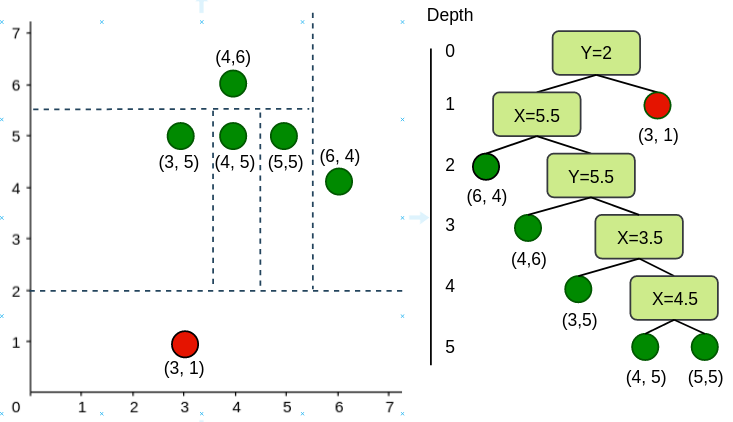
\includegraphics[width=\linewidth]{images/rich_sketch_original.png}
  \caption{}
  \label{fig:rich_sketch_original}
\end{figure}